% !TEX encoding = UTF-8
% !TEX TS-program = pdflatex
% !TEX root = ../tesi.tex

%**************************************************************
\chapter{Missing features and future developments}
\label{cap:future-developments}
%**************************************************************.

This chapter will illustrate the missing features, the limitations of the implemented architecture, the 
possible optimizations that can be implemented and future developments for the project as a whole.

%**************************************************************

\section{Missing features}

In this section we introduce the missing features for a complete implementation of the \textit{Stipula} 
language. The reason for the lack of these features is not due to a limitation of the built architecture, 
but due to a lack of time to implement them.

\subsection{Language features not implemented in the current version}

The language offers several features for writing contracts. Many of these features require certain 
properties to be guaranteed, which are often complex to maintain. In the architecture illustrated above, all 
the features of the language have been implemented, except one: the sending of messages from the contract to 
the customer. The original example of the \verb|BikeRental| contract (see section 
\ref{bike-rental-example-definition}) foresaw:
\begin{enumerate}
  \item When the user called the \verb|accept| function, the bicycle code was sent to the customer. In 
  particular, the complete code would have been:
  \label{send-use-code}
  \begin{Verbatim}[numbers=left,xleftmargin=2cm,firstnumber=14]
    ...
    @Proposal Borrower : accept()[y]
        (y == cost) {
            y -o wallet;
            use_code -> Borrower
            ...
  \end{Verbatim}
  \item When the \verb|accept| function is required was executed, the contract would notify the customer of 
  the end of the service, by sending the \verb|"End_Reached"| message. In particular, the complete code 
  would have been:
  \label{trigger-event-with-message}
  \begin{Verbatim}[numbers=left,xleftmargin=2cm,firstnumber=18]
    ...
    now + rentingTime >>
      @Using {
        "End_Reached" -> Borrower
        wallet -o Lender
      } => @End
    ...
  \end{Verbatim}
\end{enumerate}

The architecture is ready to implement this feature, that is, the infrastructure for communication between 
the virtual machine and the client has already been implemented. The missing part is figuring out the 
necessary data structures and response messages to send to the client.

\label{syntactic-sugar}
Due to time constraints, it was not possible to implement the \textit{syntactic sugar} required by the 
language. The language expects the following syntactic sugar:
\begin{enumerate}
  \item 
  \begin{Verbatim}[xleftmargin=2cm]
    ...
    @State1,@State2 Party1,Party2 : functionName()[]
    ...
  \end{Verbatim}

  That is, allowing a specific function to be called from multiple parties and/or from multiple states. The 
  implementation of this syntactic sugar involves both the compiler and the virtual machine: the compiler 
  must produce optimized bytecode, that is, instead of writing the function body for each state and for each 
  party, one could update the bytecode language to notify the virtual machine that that code can be invoked 
  from different parties and in different states. The benefits would be obtained from the point of view of 
  memory, as it would be possible to save space instead of duplicating the body of the function each time. 
  In a distributed context, this represents an important point, because it is important to minimize memory 
  usage as much as possible. It is necessary to clarify this is a pure consideration from the point of 
  view of optimization and not from the point of view of expressiveness. The lack of this syntactic sugar 
  does not diminish the expressiveness of the language: in fact, it is possible to write the same function 
  code several times in the bytecode with different states and callers. However, the implementation of 
  this syntactic sugar was not possible due to lack of time.
  \item See \cite{site:stipula-programming-legal-contracts}
  \begin{Verbatim}[xleftmargin=2cm]
    ...
    ~ @End _ : block(x) {
      x -> _
    } ==> @Exception
    ...
  \end{Verbatim}

  Similarly to the previous point, the implementation of this syntactic sugar involves the compiler and the 
  virtual machine. The meaning of this code is as follows: the \verb|block| function can be invoked by any 
  party ("\verb|_|" notation) provided that the duration of the contract has not expired, that is, the 
  contract is not in the \verb|@End| state.
\end{enumerate}

\subsection{Single-use-seals merge}
\label{single-use-seals-merge}

The current version has an important limitation when the user has to make a payment to an instance of a 
contract. In order to make a payment, the user must have available a single-use-seal of the exact quantity 
required by the contract: if the user does not have a single-use-seal of the requested quantity, the user 
cannot make the payment. This problem represents a strong limit to be able to massively use this 
implementation. One proposed solution is to \textit{merge} single-use-seals. Suppose Alice has to pay the 
contract \verb|C_1| 15 \verb|StipulaCoin|. Alice has the following single-use-seals available (note the 
image \ref{fig:single-use-seals-merge}):
\begin{enumerate}
  \item Single-use-seal 1 (\verb|S_1|): 5 \verb|StipulaCoin|;
  \item Single-use-seal 2 (\verb|S_2|): 7 \verb|StipulaCoin|;
  \item Single-use-seal 3 (\verb|S_3|): 2 \verb|StipulaCoin|;
  \item Single-use-seal 4 (\verb|S_4|): 2 \verb|StipulaCoin|;
\end{enumerate}

\begin{figure}[htbp]
	\begin{center}
		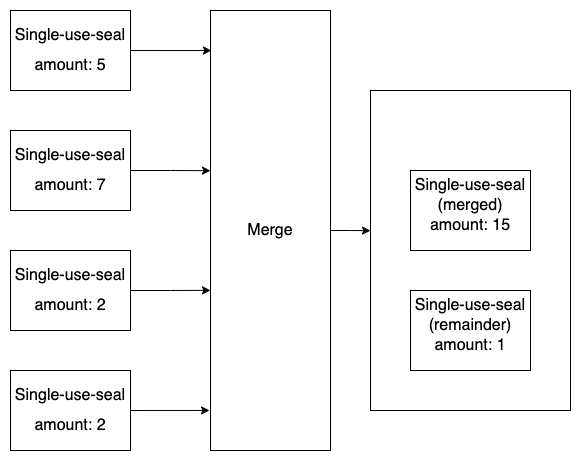
\includegraphics[height=7cm]{immagini/capitolo-6/single-use-seals-merge.png}
		\caption{Example of single-use-seals merge.}
		\label{fig:single-use-seals-merge}
	\end{center}
\end{figure}

In the current version Alice could not pay the contract as she does not have a single-use-seal of 15 
\verb|StipulaCoin|, however the sum of all available funds is 16 \verb|StipulaCoin|, enough to be able to 
carry out the transaction. The proposed solution consists first of all in modifying the message to make 
function calls (see \ref{function-call-message}), specifically when a \textit{Pay-to-Contract} must be 
made. The message must be able to collect multiple single-use-seals in its payload. More precisely:
\begin{enumerate}
  \item \verb|unlockScript| must be provided for each single-use-seals, so that the user proves ownership of 
  the funds;
  \item Create new single-use-seals:
  \begin{enumerate}
    \item One represents the single-use-seal that will be sent to the contract (\verb|merged|); % line 58
    \item The other single-use-seal represents the \textit{remainder} (\verb|remainder|), that is, 
    the difference between the sum of all the single-use-seals in input minus the amount of asset needed to 
    contract. % line 72
  \end{enumerate}
\end{enumerate} 

I single-use-seals \verb|merged| and \verb|remainder| are the new single-use-seals that will need to be 
stored. The identifier of these single-use-seals is computed from the hash of the input single-use-seals 
identifiers. The reason is to decrease the probability of collision between the identifiers of the other 
single-use-seals. The \verb|merged| must be sent with the contract and therefore \verb|unlockScript| must be 
provided, to demonstrate possession of the single-use-seal. Instead, you don't need to supply 
\verb|unlockScript| for the \verb|remainder|, as it is not to be spent in this transaction.

An example is shown below:

\begin{enumerate}
  \item Line 5 specifies that the payment is a \textit{single-use-seal merge} (\verb|merge|). From line 8 
  to line 29, all single-use-seals that Alice wants to merge are specified. You can see that for each 
  single-use-seal, Alice has provided cryptographic proof of ownership of those funds. In particular, on 
  line 12, 17, 22, 27 it is possible to note the presence of the \verb|unlockScript| field.

  For \verb|<ownershipId_S_1>| we refer to the identifier of the \textit{first} single-use-seal that Alice 
  wants to spend and for \verb|<unlockScript_S_1>| refers to the \verb|unlockScript| del \textit{first} 
  single-use-seal. The same goes for \verb|<ownershipId_S_2>|, \verb|<ownershipId_S_3>|, 
  \verb|<ownershipId_S_4>|, \verb|<unlockScript_S_2>|, \verb|<unlockScript_S_3>| and 
  \verb|<unlockScript_S_4>|
  \begin{Verbatim}[numbers=left,xleftmargin=1cm,firstnumber=1,breaklines=true,tabsize=2]
    ...
    "arguments": [
      {
        "argument": {
          "first": "merge",
          "second": "y",
          "third": {
            "input": [
              {
                "ownershipId": "<ownershipId_S_1>",
                "address": "<Alice_address>",
                "unlockScript": "<unlockScript_S_1>"
              },
              {
                "ownershipId": "<ownershipId_S_2>",
                "address": "<Alice_address>",
                "unlockScript": "<unlockScript_S_2>"
              },
              {
                "ownershipId": "<ownershipId_S_3>",
                "address": "<Alice_address>",
                "unlockScript": "<unlockScript_S_3>"
              },
              {
                "ownershipId": "<ownershipId_S_4>",
                "address": "<Alice_address>",
                "unlockScript": "<unlockScript_S_4>"
              }
            ],
  \end{Verbatim}

  \item From line 30 to line 56, it is possible to notice what is the output of the merger of the previous 
  single-use-seals (\verb|output|). From line 31 to line 45, you can see the specification of the new 
  single-use-seal \verb|merged|, which will be sent to the contract instance to make the payment. In fact, 
  this new single-use-seal already comes with the \verb|unlockScript| (line 43). By doing so, the contract 
  will be able to verify whether these funds will actually belong to Alice or not. Instead, from line 46 
  to line 56, it is possible to notice that a new single-use-seal (\verb|remainder|) is created which 
  represents the difference between the sum of all single-use-seals specified in \verb|input | minus the 
  amount of assets required by the contract instance. No \verb|unlockScript| needs to be supplied for this 
  single-use-seal because it must not be spent on this payment.

  For \verb|<hash(ownershipId_S_1)>| means the hash of the identifier of the first input single-use-seal 
  and for \verb|<unlockScript_hash(ownershipId_S_1)>| means the \verb|unlockScript| of this new 
  single-use-seal with identifier \verb|<hash(ownershipId_S_1)>|. The same goes for the single-use-seal 
  \verb|remainder|
  \begin{Verbatim}[numbers=left,xleftmargin=1cm,firstnumber=57,breaklines=true,tabsize=2]
      "output": {
        "merged": {
          "single_use_seal": {
            "asset_id": "stipula_coin_345",
            "amount": {
              "value": "1500",
              "decimals": "2"
            }
          },
          "ownership": {
            "ownershipId": "<hash(ownershipId_S_1)>",  
            "address": "<Alice_address>",
            "unlockScript": "<unlockScript_hash(ownershipId_S_1)>"
          }
        },
        "remainder": {
          "single_use_seal": {
            "asset_id": "stipula_coin_345",
            "amount": {
              "value": "100",
              "decimals": "2"
            }
          }
        }
      }
  \end{Verbatim}
\end{enumerate}

Let's illustrate the complete example:
\label{single-use-seal-merge-example}
\begin{Verbatim}[numbers=left,xleftmargin=1cm,firstnumber=1,breaklines=true,tabsize=2]
  ...
    "arguments": [
      {
        "argument": {
          "first": "merge",
          "second": "y",
          "third": {
            "input": [
              {
                "ownershipId": "<ownershipId_S_1>",
                "address": "<Alice_address>",
                "unlockScript": "<unlockScript_S_1>"
              },
              {
                "ownershipId": "<ownershipId_S_2>",
                "address": "<Alice_address>",
                "unlockScript": "<unlockScript_S_2>"
              },
              {
                "ownershipId": "<ownershipId_S_3>",
                "address": "<Alice_address>",
                "unlockScript": "<unlockScript_S_3>"
              },
              {
                "ownershipId": "<ownershipId_S_4>",
                "address": "<Alice_address>",
                "unlockScript": "<unlockScript_S_4>"
              }
            ],
            "output": {
              "merged": {
                "single_use_seal": {
                  "id": "<hash(S_1)>",
                  "asset_id": "stipula_coin_345",
                  "amount": {
                    "value": "1500",
                    "decimals": "2"
                  }
                },
                "ownership": {
                  "ownershipId": "<hash(ownershipId_S_1)>",  
                  "address": "<Alice_address>",
                  "unlockScript": "<unlockScript_hash(ownershipId_S_1)>"
                }
              },
              "remainder": {
                "single_use_seal": {
                  "id": "<hash(S_2)>",
                  "asset_id": "stipula_coin_345",
                  "amount": {
                    "value": "100",
                    "decimals": "2"
                  }
                }
              }
            }
          }
        }
      }
    ],
    ...
  }
  ...
}
\end{Verbatim}

This solution allows you to make payments even if you don't have single-use-seals of the precise quantity 
required by the contract. The solution requires updating the message format and carrying out further 
preliminary checks before executing the contract, namely:
\begin{enumerate}
   \item Checking the single-use-seals of inputs: in addition to verifying ownership via the 
   \textit{Script}, it is also necessary to check that the sum of the inputs is greater than or equal to the 
   quantity required by the contract;
   \item Controlling single-use-seals \verb|merged| and optionally \verb|remainder|: verify that the sum of 
   the quantities of the input single-use-seals is equal to the sum of the quantities of \verb|merged| and 
   optionally \verb|remainder|. Also, verify that the single-use-seal \verb|merged| is equal to the quantity 
   required by the contract;
\end{enumerate}

Passing these checks, the input single-use-seals will be updated in \textit{Storage} as spent. The 
single-use-seals \verb|merged| will be stored in storage directly as spent, while the single-use-seal 
\verb|remainder| is stored as unspent. At this point, the virtual machine can continue with the execution of 
the contract.

\subsection{Creation of assets and their distribution}
\label{creation-assets-and-distribution}

One of the missing aspects in the current version is the ability to create additional assets beyond the 
hard-coded one. As an example, hard-coded assets have been created for the implemented version. One of the 
peculiarities of the \textit{Stipula} language is that of being able to schedule the execution of certain 
obligations over time. This functionality could be leveraged to manage the creation, issuance and 
destruction of assets. The creation of an asset should take place by means of a special contract, separate 
from the classic contracts seen above. In this special contract, the maximum supply, the fractionability of 
the asset, the name and an identifier would be defined. However, an asset issuance mechanism could also be 
defined, such as the \textit{halving} for Bitcoin ((see \cite{site:bitcoin-mining}, 
\cite{site:bitcoin-halving} and \cite{book:mastering-bitcoin})): using the scheduling of events over time, it is possible 
to establish that periodically a certain amount of assets is entered into the system. Furthermore, it is 
also possible to define addresses for the \textit{burn} of the assets. Burning an asset is used to remove 
liquidity from circulation, thereby decreasing available supply and appreciating the asset. If you want to 
burn a certain amount of assets, you send it to a specific address where you can only deposit and not 
withdraw. In this way, it is also possible to monitor and verify the amount of burned assets.

\newpage
\section{Optimizations}
\label{optimizations}

The current architecture has mainly two bottlenecks:
\begin{enumerate}
  \item \textit{Virtual Machine}: requests to execute function calls of an instance of a contract or the 
  execution of a time-scheduled event are computed \textit{sequentially};
  \item \textit{Storage}: for simplicity in the realization of the implementation, each request, both for 
  reading and for writing, is managed by a \textit{mutex}, to guarantee exclusive access to the memory by a 
  superior module .
\end{enumerate}
Requests addressed to the compiler and requests addressed to the virtual machine are handled in parallel 
until one has to interact with the \textit{Storage} module.

\subsubsection{Virtual Machine}

Requests directed to the virtual machine are done \textit{sequentially}. Unfortunately, this implementation 
choice represents a bottleneck as regards system performance, in particular, precisely for the virtual 
machine, which is the most used module during the execution of a contract. However, it is possible to 
implement optimizations, paying attention, however, to avoid cases of competition. Some possible 
optimizations for the virtual machine are:
\begin{enumerate}
  \item \textit{Parallelization of single-use-seals}: this is possible thanks to the UTXO model used in the 
  architecture. The operation of this property has been described \ref{utxo-parallelization}. For example: 
  Alice has two single-use-seals \verb|S_1| and \verb|S_2| and she wants to make two payments to two 
  different contracts \verb|C_1| and \verb|C_2|. With this optimization, Alice can pay the \verb|C_1| 
  contract with \verb|S_1| and \verb|C_2| with \verb|S_2|. The two requests can be run in parallel because 
  they use separate funds and there is no need to run either request first to update the asset balance, as 
  might be the case in an account-balance-based model. The same dynamic would also occur if Alice had to 
  pay two different instances of the same contract or two instances of two different contracts;
  \item \textit{Parallelization of function calls}: if a user is interacting with multiple instances of 
  contracts at the same time, the requests can be executed in parallel. If multiple users are interacting 
  with the same instance of a contract, requests will be fulfilled in order of arrival. As regards the 
  execution of obligations (events scheduled over time), the basic principle does not change: the event 
  can be parallelized if the other requests interact in different contract instances, otherwise the 
  execution of the event has priority over the execution of function calls.
\end{enumerate}

These optimizations can significantly increase the \textit{throughput} of requests, especially in a 
distributed context. However, it is necessary to update the structure of some modules and to pay particular 
attention to concurrency.

\subsubsection{Storage}

Requests received by this module could be parallelized by splitting them into \textit{read} and 
\textit{write} requests. Requests can come from the compiler, from the virtual machine or directly from the 
\textit{Message Service}. If the module is only receiving read requests, these requests can be executed in 
parallel; when a write request is received, it takes priority over read requests. As a further optimization, 
you could make a specific resource exclusive when a write request is received, and leave free access to 
other resources.

\section{Limits of the architecture}

\subsection{Computational and memory resources required}

One of the factors to increase the decentralization of a network is to allow the creation of nodes that 
have a low computational capacity and limited storage capacity. If a ledger were to require large 
computational capabilities and large amounts of memory, this implies that more expensive machines would be 
needed. The need for more expensive machines increases the centralization of the network, as the subjects 
who will be able to buy and maintain these machines will be limited in number. Therefore, in the design 
phase it is also important to take into account the computational and memory aspect. One of the most 
expensive operations in a decentralized network is the \textit{synchronization} of the nodes. If the ledger 
used a lot of memory, this would increase the time it takes to synchronize, thus increasing the possibility 
of transmission errors. Obviously, this phase would be much more complex and difficult to complete for 
devices with limited computational and memory capabilities. The current implementation stores various 
information in the \textit{Storage} module. This could pose a problem for especially distributed networks, 
if decentralized. During the development of the project we focused on saving all the information necessary 
to allow the execution of the contracts and for the management of the asset transfers. It would be necessary 
to analyze whether all the information that is currently stored is actually necessary or, on the other hand, 
it is possible to omit some information because it is possible to deduce it from other information. 
Obviously, this balance must be calibrated correctly with the computational cost required to retrieve this 
information: if it is possible to save a minimal set of information that is currently stored, but the 
operations necessary to retrieve it require a considerable increase in computational resources, this 
represents one downside. Furthermore, for simplicity and for a limited amount of time available, the 
information has been stored according to the data structures of Java objects, as the \textit{LevelDB} 
library allows information to be stored in bytes. A necessary development is to create information storage 
interfaces for the various storages (\textit{contracts}, \textit{contract-instances}, \textit{assets} and 
\textit{ownerships}), in order to allow to implement nodes also in other programming languages.

From a computational point of view, the current version of the language is not Turing-complete, so it is not 
possible to loop and make function calls from other functions. This design choice limits the expressiveness 
of the language and therefore also limits the possibility of creating programs that may require significant 
computational resources. The \textit{Script} language is also not Turing-complete, so it is possible to 
create programs that require little computational resources. Furthermore, non-Turing-completeness also 
allows you to avoid unwanted behavior and prevent potential security vulnerabilities. In the previous 
section (\ref{optimizations}), possible optimizations were introduced to increase request throughput. These 
optimizations must also take into consideration devices that have limited computational capacity: in this 
case it is preferable to implement certain optimizations and others not, obtaining a lower throughput for 
greater decentralization. Obviously, these considerations refer exclusively to decentralized networks.

\newpage
\section{Current version security issues}

One of the key principles that guided the entire development is security from various points of view. In 
fact, security can be understood as regards:
\begin{enumerate}
   \item The assets, that is, guaranteeing that the transfer of assets between users and contracts, and vice 
   versa, takes place without loss of quantity or generation of new quantities from scratch;
   \item Prevent a user from double-spending;
   \item Ensure that after a contract is executed, the correct state is reached.
\end{enumerate}

The architecture presented above has a security problem regarding the transmission of messages between the 
server/node and the client. The attack that might occur is a \textit{Man-In-The-Middle} (\textit{MITM}) 
attack. When a user wants to send a message to the \textit{Stipula} server/node, the message is signed. The 
benefits of signing are:
\begin{enumerate}
   \item \textit{Authentication}: the recipient can verify that the message was sent by the declared sender, 
   since only the sender has the private key to sign the message;
   \item \textit{Integrity}: the recipient can be certain that the message has not been tampered with during 
   transmission, as any alteration of the message would invalidate the signature;
   \item \textit{Non-repudiation}: the sender cannot deny having sent the message once signed, since the 
   signature provides verifiable proof of authorship.
\end{enumerate}

Thus, when the \textit{Stipula} server/node receives a message, even if it is not encrypted, the sender has 
expressed his intentions of wanting to create a new instance of a contract or make a function call. However, 
when it is the \textit{Stipula} server/node that has to send response messages to the client, these can be 
intercepted and tampered with. Indeed, in the server/node there are no cryptographic keys that certify the 
authenticity and integrity of a message. The problems of having cryptographic keys inside a server/node are:
\begin{enumerate}
   \item If the cryptographic keys are found by an attacker, the latter can send malicious messages to users;
   \item If the keys are lost and a new pair is generated, the problem described in the previous point would 
   arise: the user could not think that the keys have been changed by an attacker and therefore could think 
   that they are receiving malicious messages.
\end{enumerate}

However, in a distributed and centralized context, the use of cryptographic keys in the nodes could be a 
sufficiently secure solution, as the control of the network belongs to a central body which monitors the 
traffic. Therefore, nodes with a cryptographic key pair and the central body would be able to cope with 
similar attacks. The problem arises in networks where there is no central body that governs the network.

You can locate the problem in some response messages:
\begin{enumerate}
   \item When the server/node has to send the response after the \textit{agreement} phase of a contract. 
   When the agreement phase takes place, the server/node creates a new instance of the contract and assigns 
   it a unique identifier. This identifier will be inserted as the response payload. An attacker could 
   intercept this message and alter it by inserting an identifier that points to an instance of a malicious 
   contract. By doing so, the user would not notice the change of identifier and would go to accept, and 
   therefore have to respect, the obligations defined in the contract uploaded by the attacker;
   \item When server/node sends additional payload in responses. Taking as an example the instruction 
   \verb|use_code -> Borrower|, previously defined in \ref{send-use-code}, the server/node should add the 
   bicycle code as payload to the response. This message could be intercepted by an attacker, replace the 
   bike code with a fake one, and keep the original bike code. At this point the user would not be able to 
   use the service, as the code is not the original one and if the situation were not resolved before the 
   penalty is triggered, i.e. the trigger of the event previously defined in 
   \ref{trigger-event-with-message}, the contract will send all the money to the company.
\end{enumerate}

We are aware of the issues associated with this architecture, but it was not possible to take steps to 
mitigate these issues due to lack of time.

\section{Future improvements}

\subsection{Implementation of the consensus module and communication protocols}

This represents the most important module in the distributed context. In this module, it will be necessary to 
develop communication protocols and algorithms that make it possible to determine consensus regarding the 
result of the execution of a contract.

The design and development of this module will be very complex as it will have to take into account various 
security aspects, such as spam. A proposal to try to mitigate the phenomenon of spam is the use of 
\textbf{hashcash} \autocite{site:hashcash}, a \textit{proof-of-work} algorithm which aims to prevent 
spam and \textit{DoS} attacks (\textit {Denial-of-Service}), making it more difficult and time-consuming 
for a sender to send large volumes of requests to a service. The way hashcash works requires the sender to 
solve a computational puzzle that requires significant computational power to complete. The puzzle is to 
find a hash value that meets certain criteria, such as having a certain number of leading zeros. The sender 
has to compute many hash values until it finds one that satisfies the criteria, which takes a lot of 
computing power and time. Once the sender has solved the puzzle and found a valid hash value, they include 
this value in the request as proof of work. The recipient can then quickly verify the proof of work by 
checking the hash value, which allows them to determine whether the sender expended enough computing power 
to send the request. The power of this mechanism consists in the need for a substantial amount of time and 
energy to create a proof of work, and at the same time, the verification of the latter can be done 
instantaneously. The concept of hashcash underpins how Bitcoin proof-of-work works. A similar algorithm 
adapted to \textit{Stipula} could allow the network of nodes to limit the spam introduced by one or more 
attackers. 

Another useful consensus module component is the creation of a \textit{mempool}. When the virtual machine 
executes an instance of a contract and the execution is successful, the results produced must first be 
verified with other nodes to verify that the network (or the majority of the network) agrees with the same 
results. The network of nodes may be congested and therefore requests may not be served immediately. To free 
up the virtual machine and run other instances of contracts, it might be useful to implement a queue of 
requests to submit for consent.

\subsection{Implementation of the commitment module}

This layer allows you to communicate with an underlying layer to do the timestamping and commitment of 
information. In particular, this module will have to provide common interfaces, in order to make the 
implementation of \textit{Stipula} independent from the layer that will be used. In fact, if you want to 
use Ethereum as a commitment layer, you will have to develop specific code that allows you to interact 
directly with the blockchain, and at the same time respect the common interfaces of the \textit{Stipula} 
commitment module: in doing so the others modules of the architecture will not change. To do this, the 
modules that would be involved are:
\begin{enumerate}
  \item The \textit{Storage} module (see sections \ref{storage-module} and \ref{storage}): this module 
  will have to store inside the data that will indicate how to find the information saved in the 
  commitment layer;
  \item The \textit{Commitment} module (see section \ref{commitment-module}): this module will have to 
  interface with the underlying layer to instruct which information will have to be saved;
  \item The \textit{Communication protocols} module (see section \ref{communication-protocols-module}): 
  communication protocols will be needed between the commitment layer and the \textit{Stipula} 
  implementation for the exchange of information.
\end{enumerate}

Also in this case it is useful to implement a mempool, as the layer could be congested and consequently 
there could be slowdowns in writing the results obtained from the execution of the contracts.

\subsection{Fees for performance of a contract}

All the smart contracts of various blockchains require \textit{fees} to be paid for their execution, 
as the computational and memory resources of a distributed network are used. This also happens for layer two, 
such as \textit{Arbitrum} (see \cite{site:arbitrum} and \cite{site:arbitrum-fees}) and \textit{Optimism} 
(see \cite{site:optimism} and \cite{site:optimism-fees}) for Ethereum. Fees make possible network attacks 
(such as \textit{spam}) costly in terms of money and/or resources. Furthermore, fees are a useful tool for 
\textit{prioritizing} requests: when a blockchain is congested, the network prioritizes those transactions 
that pay more fees than the others.

The current implementation of \textit{Stipula} does not take this dynamic into consideration: if this 
version were based on a commitment layer, it is not possible to pay commissions for writing the information. 
Nor are there any commissions for the network of nodes that execute the \textit{Stipula} contracts. As a 
future development, it may be necessary to separate the payments to be made to a contract from the 
commission costs for the execution of the same, both for the network of \textit{Stipula} nodes and for a 
possible commitment layer. This problem may not arise if \textit{HyperLedger Fabric} nodes are used as 
commitment layer, which do not include commission costs for writing information in the ledger.

\subsection{Script language extension}

The advantages of using the \textit{Script} language have been described in previous chapters. By extending 
this language, it is possible to create advanced ways to spend funds, such as authorizing a transaction from 
multiple users or restricting that a certain amount of assets can only be spent after a certain date. The 
extensibility of the language makes it possible to satisfy certain needs that could arise in certain 
contexts, for example: in a corporate context, it could be useful to carry out a certain expense only with 
the authorization of several figures, such as directors or managing directors. So, extensibility also allows 
you to create new, more secure ways to manage your assets. Extensibility can be implemented by adding new 
instructions to the already existing set (see \ref{table:instructions-svm}) or modifying the current ones, 
tightening or relaxing the constraints.

\subsection{Implementation of additional software}

In order to incentivize the use of \textit{Stipula} and allow developers to build software on top of its 
implementation, it is necessary to provide a set of tools and software, such as SDKs. In particular, it is 
very useful for users to have an application that implements the functions of a \textit{wallet}, that is, a 
software that allows you to view the balance sheet for each asset, sign transactions, view all sent and 
received transactions, view the contracts it has approved and other privacy-focused features, such as 
\textit{coin selection} (\ref{coin-selection}). Another context that requires support software is that of 
writing contracts. Whoever writes the contracts will be a professional figure in the legal field and 
therefore it will be necessary to provide tools that allow for the translation of the contractual clauses 
into \textit{Stipula} code. Therefore, it could be useful to modularize the compiler and the virtual machine 
to develop tools to be integrated into the IDEs: in doing so, before loading a contract into an instance or a 
\textit{Stipula} node, the person who will write the contract will be able to check whether the written code 
will be correct and that respects the expected behaviors. Developing additional tools and software requires 
interacting only with the \textit{Message Service} module (see \ref{message-service}), as all requests and 
replies go through this module. This facilitates the work of developers, as:
\begin{enumerate}
  \item They must not interact with other modules, such as the virtual machine, whose tasks are very 
  delicate;
  \item Message formats are defined, and therefore it is possible to build tools on top of a 
  \textit{Stipula} server or node, without worrying about messages changing structure. Currently, message 
  formats may change over time until the architecture structure is solid and stable. At that point, message 
  formats will no longer have to change, but new messages can be created for new features.
\end{enumerate}
